\documentclass[main.tex]{subfiles}
\begin{document}
The continuous-time random walk model \cite{montrollweiss1965} on a graph is a
Markov process where transitions have a fixed probability per unit time,
$\gamma$, of moving to adjacent vertices. Consider a graph $G$ with $N$
vertices and no self-loops, this walk can be defined by the linear differential
equation that describes the probability of jumping to a connected vertex at any
given time 
\begin{equation}
	\frac{dp_i(t)}{dt} = \gamma \sum_j L_{ij} p_j(t), \label{eq:classicalContWalk}
\end{equation}
where $L$ is the Laplacian defined as $L = A - D$, and $p_j(t)$ is the
time-dependent probability associated with each vertex transition. $A$ is the
adjacency matrix that represents each vertex connection, given by
\begin{equation}
	A_{ij} = \begin{cases} 1, & \mbox{if } (i,j)\in G \\ 0, & \mbox{otherwise,} \end{cases}
\end{equation}
and D is the diagonal matrix $D_{jj} = deg(j)$ corresponding to the
degree
of vertex $j$.\par

\begin{figure}[!h]
	\centering
    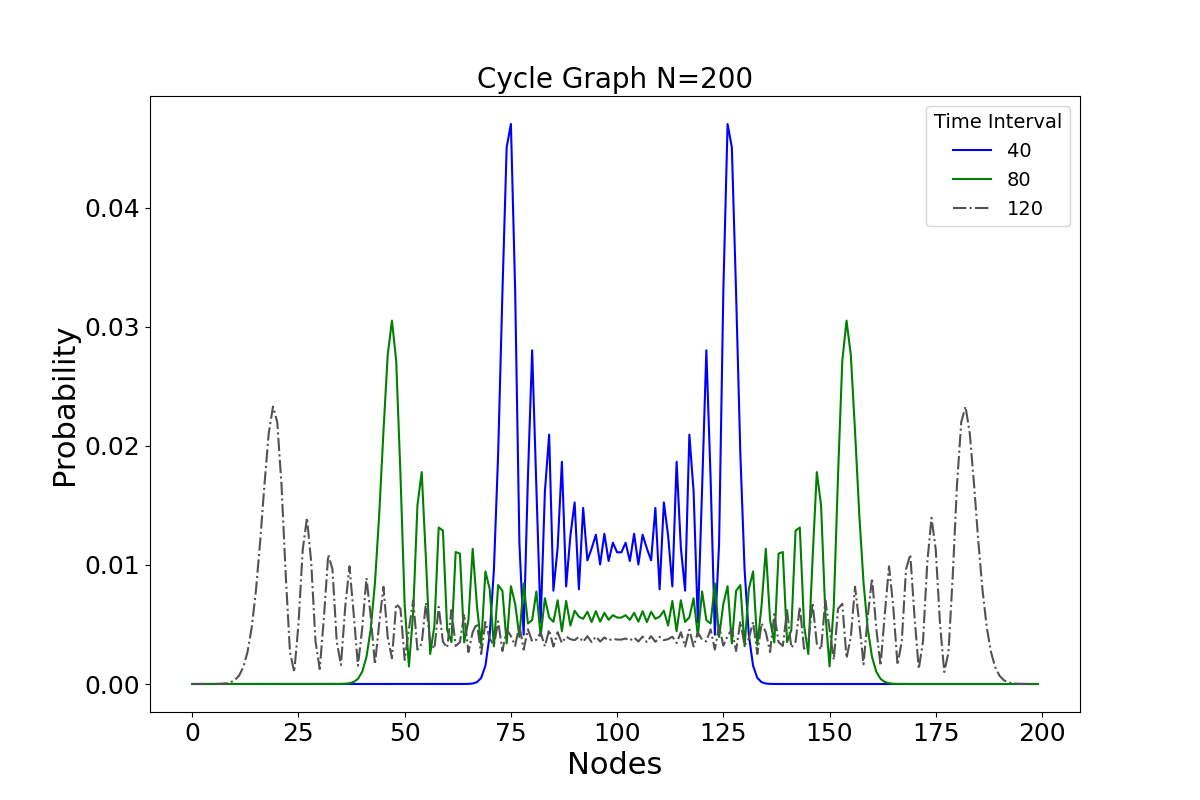
\includegraphics[scale=\mysinglefigurescale]{img/QWAK/UndirectedDynamics/cycleDynamics_N200_GAM0.354_TMAX40-80-120.png}
    \caption{Probability distribution for the CTQW on a line of size $N=200$,
    at $t=40$, $80$ and $120$, with initial condition $\ket{\psi(0)}=\ket{0}$
    and $\gamma=\frac{1}{2\sqrt{2}}$.} 
	\label{fig:contdist0}
\end{figure}

Analogously, Schrödinger's equation describes the quantum version of the walk 

\begin{equation}
	i\hbar \frac{d\ket{\psi(t)}}{dt} = H \ket{\psi(t)}, \label{shrodinger}
\end{equation}
where $H = -\gamma L$ is the Hamiltonian of the system, or simply $H = -\gamma
A$. This operator can be defined either as a time-independent Laplacian or
adjacency matrix without loss of generality. Considering $\hbar = 1$, the
solution of the continuous-time quantum walk will be 

\begin{equation}
	\ket{\psi(t)} = U(t)\ket{\psi(0)}.
    \label{eq:ctqwSystemEvolution}
\end{equation}
where $\psi(0)$ is a compatible initial condition and the unitary matrix $U(t)$
is
\begin{equation}
	U(t) = e^{-iHt} = e^{i(\gamma L)t} = e^{i\gamma(A-D)t}.
    \label{eq:contSimulUniOp}
\end{equation}

A brief look at Figure \ref{fig:contdist0} highlights key properties of the
quantum walk. Contrary to the classical scenario, where the probability of
finding the walker is predominantly concentrated around the origin with a
standard deviation scaling as $\sqrt{t}$ (termed \textit{diffuse} propagation),
the quantum walk exhibits \textit{ballistic} propagation, proportional to $t$. Here, the probability
peaks away from the origin, and the standard deviation grows linearly with time
\cite{childs2002}, indicating a quadratic advantage in the quantum case.

\end{document}
